\def\levelsep{.7} %
\def\nodesep{.7}  %

\footnotesize
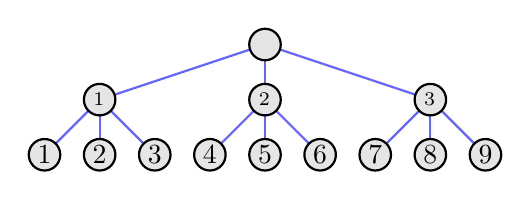
\begin{tikzpicture}
    [vertex/.style={circle, draw=black, fill=black!10!white, thick, inner sep=0pt, minimum size=4mm, align=center},
        new/.style={draw=red, fill=red!30!white},
        exclude/.style={fill=red!40!white},
        tree/.style={draw=blue!60!white, thick},
        label/.style={right=4pt}]

\coordinate (a) at (4 * \nodesep, \levelsep);
\coordinate (b) at (1 * \nodesep, 0);
\coordinate (c) at (4 * \nodesep, 0);
\coordinate (d) at (7 * \nodesep, 0);
\coordinate (e) at (0 * \nodesep, -\levelsep);
\coordinate (f) at (1 * \nodesep, -\levelsep);
\coordinate (g) at (2 * \nodesep, -\levelsep);
\coordinate (h) at (3 * \nodesep, -\levelsep);
\coordinate (i) at (4 * \nodesep, -\levelsep);
\coordinate (j) at (5 * \nodesep, -\levelsep);
\coordinate (k) at (6 * \nodesep, -\levelsep);
\coordinate (l) at (7 * \nodesep, -\levelsep);
\coordinate (m) at (8 * \nodesep, -\levelsep);

\draw[tree] (a)--(b);
\draw[tree] (a)--(d);
\draw[tree] (b)--(e);
\draw[tree] (b)--(f);
\draw[tree] (d)--(k);
\draw[tree] (d)--(m);
\draw[tree] (a)--(c);
\draw[tree] (b)--(g);
\draw[tree] (c)--(h);
\draw[tree] (c)--(j);
\draw[tree] (c)--(i);
\draw[tree] (d)--(l);

\node[vertex] at (a) {$\nr$};
\node[vertex] at (b) {$\nin_1$};
\node[vertex] at (c) {$\nin_2$};
\node[vertex] at (d) {$\nin_3$};
\node[vertex] at (e) {$\nleaf{1}$};
\node[vertex] at (f) {$\nleaf{2}$};
\node[vertex] at (g) {$\nleaf{3}$};
\node[vertex] at (h) {$\nleaf{4}$};
\node[vertex] at (i) {$\nleaf{5}$};
\node[vertex] at (j) {$\nleaf{6}$};
\node[vertex] at (k) {$\nleaf{7}$};
\node[vertex] at (l) {$\nleaf{8}$};
\node[vertex] at (m) {$\nleaf{9}$};

\end{tikzpicture}
